\chapter{Aberration Correction in for Spinning Disk Confocal Microscopy}
\label{chpt:Aurox}

\section{Image Formation in Aurox Clarity Module}
\label{sec:Aurox_image_formation}

Figure~\ref{fig:confocal_schematic} shows a simplified schematic 
for a Nipkow-Petran spinning disk confocal microscope. The 
excitation illumination passes through aperture mask, which is 
then imaged onto the sample. This aperture mask consists of a 
number of pinholes packed closely together, illumating a number 
of focal spots at once. The excitation light then passes back 
through the aperture mask where the out-of-focus light is 
discarded by the pinhole array.\cite{egger1967new,fuseler2018types}

\begin{figure}[h]
	\centering
	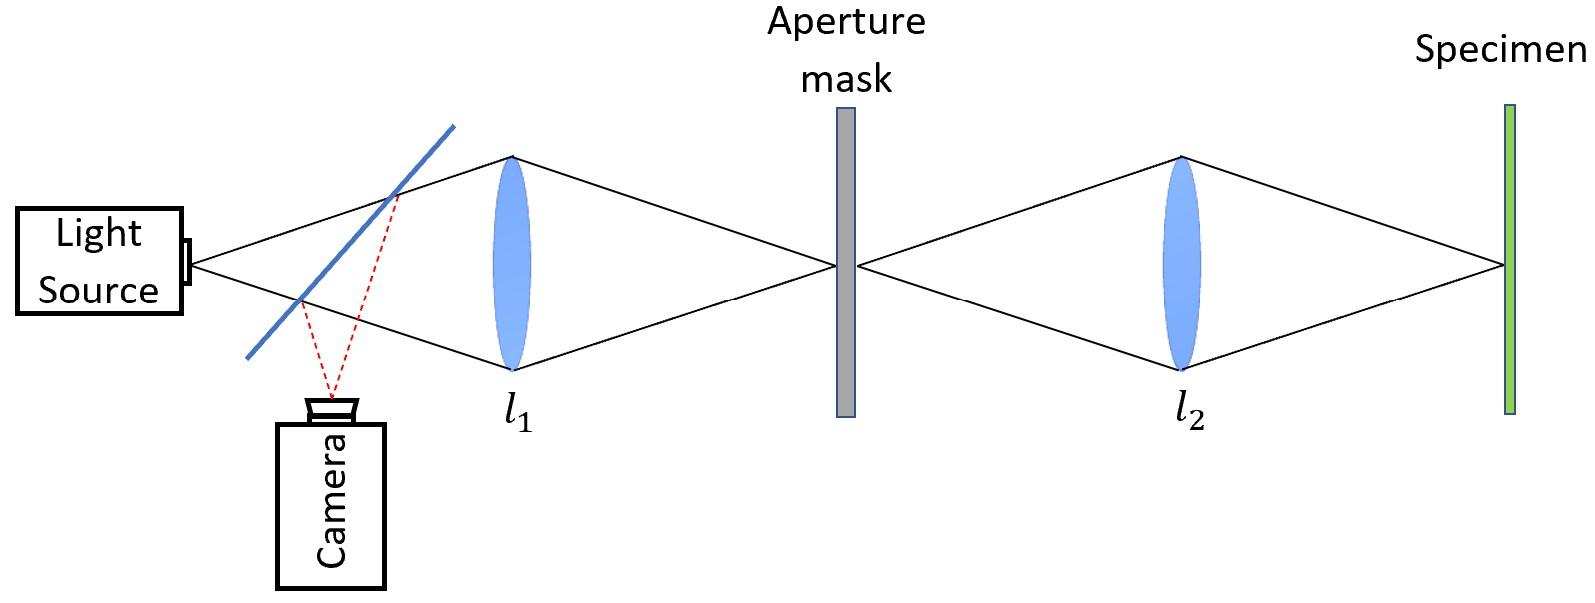
\includegraphics[width=\textwidth]{images/confocal_schematic.jpg}
	\caption{A schematic diagram showing a simplified layout for a Nipkow-Petran spinning disk confocal microscope}
	\label{fig:confocal_schematic}
\end{figure}

Consider a transmissive optical system as shown in 
Figure~\ref{fig:optical_system_schematic}. For an incoherent 
light source, immediately after the detector mask the 
intensity, $I\left(\textbf{x}_{2}\right)$, is given by:

\begin{equation}\label{eq:intensity_after_detector}
	I\left(\textbf{x}_{2}\right) = \int S\left(\textbf{x}_{1}\right) D\left(\textbf{x}_{2}\right) \left| \int h_{1}\left(\textbf{x}_{0} + \frac{\textbf{x}_{1}}{M}\right) \tau\left(\textbf{x}_{0}\right) h_{2}\left(\textbf{x}_{0} + \frac{\textbf{x}_{2}}{M}\right)d\textbf{x}_{0}\right|^{2}d\textbf{x}_{1}
\end{equation}

Where $S\left(\textbf{x}_{1}\right)$ is the intensity 
sensitivity of the source mask, $D\left(\textbf{x}_{2}\right)$ 
is the detector mask, $\tau\left(\textbf{x}_{0}\right)$ is 
the amplitude transmittance function of the aperture mask, 
$h_{1}$ and $h_{2}$ are the amplitude point spread functions 
(PSFs) of the two imaging lenses respectively and $M$ is the 
magnification factor. 

\begin{figure}[h]
	\centering
	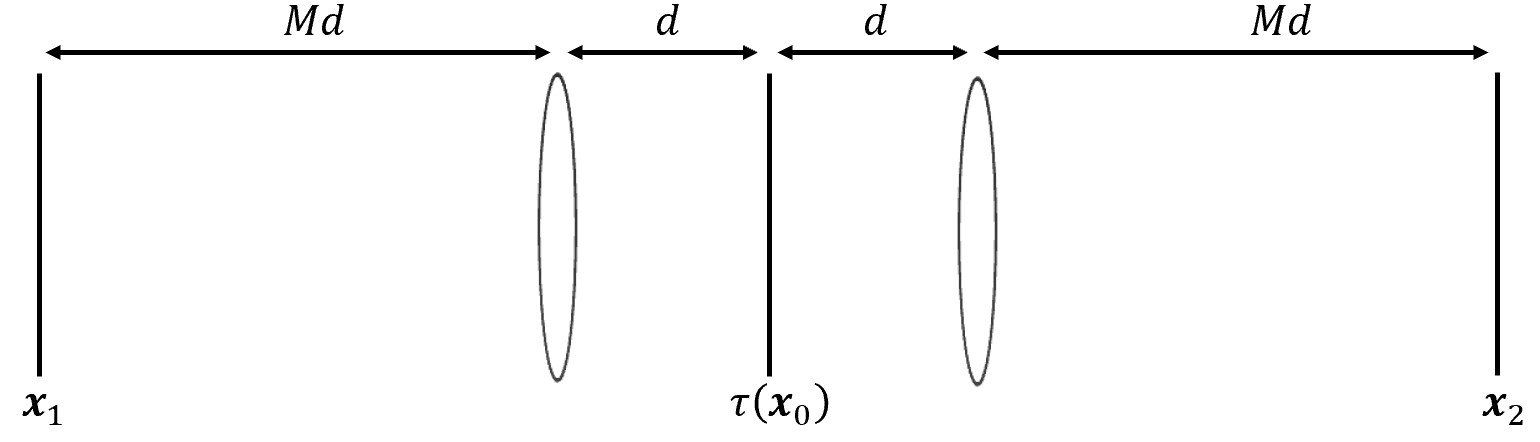
\includegraphics[width=\textwidth]{images/optical_system_schematic.jpg}
	\caption{A simple schematic diagram of a transmissive optical system}
	\label{fig:optical_system_schematic}
\end{figure}

Consider the case of reflection just after the detector mask 
and with the detector aperture positioned at some 
$\textbf{x}_{i}$ such that $S\left(\textbf{x}\right) = 
D\left(\textbf{x}\right) = \delta\left(\textbf{x} - 
\textbf{x}_{i}\right)$, where here $\delta$ denotes the Dirac 
delta function. In this case, assuming an ideal point source, 
the intensity at $\textbf{x}_{i}$ from 
Equation~\ref{eq:intensity_after_detector} becomes:

\begin{equation}\label{eq:confocal_image_form}
	I\left(\textbf{x}_{i}\right) = \left| \int h_{1}\left(\textbf{x}\right) h_{2}\left(\textbf{x}\right) \tau\left(\textbf{x} - \frac{\textbf{x}_{i}}{M}\right)d\textbf{x}\right|^{2}
\end{equation}

Which is the equation which describes image formation in 
conventional confocal microscopes.\cite{wilson1990confocal} 
This describes the image formation from a single point source 
and hence requires scanning in $\textbf{x}_{i}$ to form a 
complete image of the field of view of the object. To remove 
the need for scanning, the source and detector masks should 
instead be composed of an array of pixels with variable 
transmittence where each pixel's transmittence is time 
dependent, $b_{i}\left(t\right)$. The source and detector 
masks can then be described by:

\begin{equation}\label{eq:detector_aperture_time}
	S\left(\textbf{x}\right) = D\left(\textbf{x}\right) = \sum_{i=0}^{N} b_{i}\left(t\right)\delta\left(\textbf{x} - \textbf{x}_{i}\right)
\end{equation}

Where $N$ is the number of pixels and each pixel has a 
coordinate $\textbf{x}_{1}, \textbf{x}_{2},...,\textbf{x}_{N}$. 
The resultant image is given by the time average of 
Equation~\ref{eq:intensity_after_detector}:

\begin{equation}\label{eq:confocal_image_time_ave}
	\left\langle I\left(\textbf{x}_{2}\right)\right\rangle = \left\langle \int S\left(\textbf{x}_{1}\right) D\left(\textbf{x}_{2}\right) \left| \int h_{1}\left(\textbf{x}_{0} + \frac{\textbf{x}_{1}}{M}\right) \tau\left(\textbf{x}_{0}\right) h_{2}\left(\textbf{x}_{0} + \frac{\textbf{x}_{2}}{M}\right)d\textbf{x}_{0}\right|^{2}d\textbf{x}_{1}\right\rangle
\end{equation}

Where $\left\langle . \right\rangle$ is the time average. 
Since the only time-dependent components are 
$S\left(\textbf{x}_{1}\right)$ and $D\left(\textbf{x}_{2}\right)$ 
only the time average of 
$S\left(\textbf{x}_{1}\right) D\left(\textbf{x}_{2}\right)$ 
need be considered:

\begin{equation}\label{eq:SD_time_ave}
	\left\langle S\left(\textbf{x}_{1}\right) D\left(\textbf{x}_{2}\right)\right\rangle = \sum_{i=0}^{N}\sum_{j=0}^{N} \left\langle b_{i}\left(t\right) b_{j}\left(t\right)\right\rangle \delta\left(\textbf{x}_{1} - \textbf{x}_{i}\right) \delta\left(\textbf{x}_{2} - \textbf{x}_{j}\right)
\end{equation}

The transmittence of each pixel should be entirely 
uncorreleted with the transmittence of any other pixel. 
Therefore, a sequence of transmittences is chosen such that:

\begin{equation}\label{eq:pixel_uncorrelation}
	\left\langle b_{i}\left(t\right) b_{j}\left(t\right)\right\rangle = \delta_{ij}
\end{equation}

Where $\delta_{ij}$ is the Kronecker delta. $b_{i}\left(t\right)$ 
can therefore be any orthonormal sequence, such as an infinite, 
random sequence of $\pm1$ or finite-length complementary Golay 
sequence.\cite{golay1949multi} Unfortunately, such sequences 
require negative transmittence values which is optically 
achievable. By adding a DC shift this limitation can be overcome 
and the pixel transmissivities become:

\begin{equation}\label{eq:detector_aperture_time_DC}
	S\left(\textbf{x}\right) = D\left(\textbf{x}\right) = \frac{1}{2} \sum_{i=0}^{N} \left[b_{i}\left(t\right) + 1\right]\delta\left(\textbf{x} - \textbf{x}_{i}\right)
\end{equation} 

So the pixel transmissivities, $\left[b_{i}\left(t\right) + 
1\right]$, alternate between $0$ and $1$ as $b_{i}\left(t\right)$ 
varies between $\pm1$. Imposing the additional requirement that 
$\left\langle b_{i}\left(t\right) \right\rangle = 0$, then 
Equation~\ref{eq:SD_time_ave} becomes:

\begin{equation}\label{eq:SD_time_ave_DC}
	\begin{split}
		\left\langle S\left(\textbf{x}_{1}\right) D\left(\textbf{x}_{2}\right)\right\rangle &= \frac{1}{4} \sum_{i=0}^{N}\sum_{j=0}^{N} \left\langle \left[b_{i}\left(t\right) + 1\right] \left[b_{j}\left(t\right) + 1\right] \right\rangle \delta\left(\textbf{x}_{1} - \textbf{x}_{i}\right) \delta\left(\textbf{x}_{2} - \textbf{x}_{j}\right)\\
		&= \frac{1}{4} \left[\sum_{i=0}^{N} \delta\left(\textbf{x}_{1} - \textbf{x}_{i}\right) \delta\left(\textbf{x}_{2} - \textbf{x}_{i}\right) + \sum_{i=0}^{N}\sum_{j=0}^{N} \delta\left(\textbf{x}_{1} - \textbf{x}_{i}\right) \delta\left(\textbf{x}_{2} - \textbf{x}_{j}\right)\right]\\
	\end{split}
\end{equation}

Substituting Equation~\ref{eq:SD_time_ave_DC} into Equation~\ref{eq:confocal_image_time_ave} 
yeilds two terms. The first term is the same form as 
Equation~\ref{eq:confocal_image_form} i.e. a conventional 
confocal image. The second term is a non-confocal image 
where all the pixel transmissivities are the same. At the 
limit, where all pixels are adjacent and there is no space 
inbetween them, then $S\left(\textbf{x}\right) = 
D\left(\textbf{x}\right) = \Sigma_{i=1}^{N}\delta\left(
\textbf{x} - \textbf{x}_{i}\right) = 1$ i.e. a purely 
conventional image.\cite{juskaitis1996efficient,wilson1996confocal}. 
Therefore the image formed by the transmitted light, $I_{T}$, 
is a composite of a conventional and confocal image:

\begin{equation}\label{eq:transmitted_image}
	I_{T} = I_{conf} + I_{conv}
\end{equation}

Where $I_{conf}$ and $I_{conv}$ are the confocal and 
conventional images respectively. Instead of an array of 
pixels with programmable transmissivity, the Aurox Clarity 
module implements a disk with a photolithographed 
transmittence sequence. In this case, the transmittence 
pattern presented to a given fixed pixel is equivalent to 
the transmittence pattern along the corresponding arc of 
the disk.\cite{wilson1996confocal} 
Equation~\ref{eq:detector_aperture_time_DC} should therefore 
be modified to:

\begin{equation}\label{eq:detector_aperture_arc}
S\left(\textbf{x}\right) = D\left(\textbf{x}\right) = \frac{1}{2} \sum_{i=0}^{N} \left[b_{i}\left(\textbf{x}_{r}\right) + 1\right]\delta\left(\textbf{x} - \textbf{x}_{i}\right)
\end{equation}

Where $\textbf{x}_{r}$ is the rotation coordinate. In 
this case, the final image is obtained by averaging over 
$\textbf{x}_{r}$ rather than over time, but the result is 
still Equation~\ref{eq:transmitted_image}. Previous 
implementations of this approach acquired two images, the 
second of which had $b_{i}\left(\textbf{x}_{r}\right) = 1$ 
i.e. no aperture mask. As Figure~\ref{fig:aurox_clarity_internal} 
shows, the Aurox clarity module images both the light 
transmitted through the spinning disk and the light 
reflected off the disk where the transmissivity is $0$. In 
this case, the detector mask is defined as:

\begin{equation}\label{eq:detector_aperture_arc_reflect}
	D\left(\textbf{x}\right) = \frac{1}{2} \sum_{i=0}^{N} \left[1 - b_{i}\left(\textbf{x}_{r}\right)\right]\delta\left(\textbf{x} - \textbf{x}_{i}\right)
\end{equation}

Applying the same average over $\textbf{x}_{r}$ as before, 
the image formed by the reflected light, $I_{R}$, is:

\begin{equation}\label{eq:reflected_image}
	I_{R} = I_{conv} - I_{conf}
\end{equation}

Therefore, both the confocal and conventional images can 
be recovered by:

\begin{equation}\label{eq:confocal_image}
	I_{conf} = \frac{1}{2}\left(I_{T} - I_{R}\right)
\end{equation}

\begin{equation}\label{eq:conventional_image}
I_{conv} = \frac{1}{2}\left(I_{T} + I_{R}\right)
\end{equation}

This has the benefits of only requiring one exposure for 
the sample to acquire a confocal image and using all of 
the emitted fluorescence light. The spinning disk in the 
Clarity module has three different grid patterns with 
different spacing. The spacing of the grid pattern determines
the degree of optical sectioning and so these grid patterns
represent low, medium and high optical sectioning.\cite{neil1997method}

\subsection{Aberrations and Image Formation}
\label{subsec:Aurox_aberrations}

Section~\ref{sec:aberrations} has already discussed the origin of 
optical aberrations and their effect on image formation for 
conventional imaging techniques. Such effects are still relevent
and degrade the image quality in the Aurox Clarity system. In addition,
in the excitation path aberrations have the effect of bluring the 
disk image on the sample which results in a loss of contrast and 
axial resolution due to reduction in spatial frequency
information.\cite{wilson1990confocal, hell1993aberrations} In the 
emission path, the fluorescence signal of the sample is similarly
degraded leading to a reduction of the signal in both $I_{T}$ and
$I_{R}$, hence a reduction in the SNR of $I_{conf}$. 

\section{Biological Exemplar}
\label{sec:Aurox_biology}

To demonstrate the improvement in image quality adaptive optics
provides in the Aurox Clarity system, we utilise two samples from
\textit{Drosophila melanogaster}; neuro-muscular junctions, NMJ, 
and egg chambers.

\subsection{Sample preperation}
\label{subsec:Aurox_sample_prep}

\subsubsection{Neuro-muscular Junction}
\label{subsubsec:Aurox_NMJ_prep}
	
The \textit{Drosophila melanogaster} neuro-muscular junction, NMJ, 
samples were prepared by following the protocol. 
3rd instar \textit{Drosophila melanogaster} larvae (Oregon-R 
strain) were dissected in HL3 buffer with $0.3mM~\text{Ca}^{2+}$ to 
prepare a larval fillet. After this, larvae were fixed with 
paraformaldehyde and blocked using BSA. Larvae were stained 
overnight with Horseradish Peroxidase, HRP, conjugated to Alexa 568 
fluorophore to visualise the neurons, and primary mouse antibody 
against Discs large, DLG, to visualise the postsynaptic density. 
The next day, the larvae were counterstained with secondary 
antibody to detect the DLG (donkey anti-mouse conjugated to 
Alexa 488 fluorophore was used), as well as DAPI to visualise the 
nuclei. The larvae were then washed and mounted in 65\% 
vectashield.\cite{brent2009drosophila} This dilution of 
vectashield is compatible with the AMEP4694 $60\times$ oil 
immersion lens.

\subsubsection{Egg chambers}
\label{subsubsec:Aurox_Egg_chambers_prep}

The \textit{Drosophila melanogaster} egg chamber samples were 
prepared by following the protocol. Ovaries were isolated from 
\textit{Drosophila melanogaster} adult females straight into fixation 
medium and fixed in 4\% PFA (prepared fresh from a stock solution 
of 16\% paraformaldehyde, methanol free ultra - pure EM grade, 
Polysciences) in Cytoskeleton Buffer for 10 minutes without added 
detergent.\cite{jia2016automatic,zhang2020nanoscale,leyton2016pfa} 
Ovaries were then heptane permeabilised and post fixed in 4\% PFA 
in PBS for not more than 15 minutes, then washed three times with 
PBS/TX-100, 0.05\%. Actin was labelled with Phalloidin Alexa 488 
(Phalloidin: stock 200 units/ml in Methanol, 6.6 $\mu$M) at between 
5 and 20 $\mu$l stock in 200 $\mu$l for at least 45 min at RT (or 
O/N at $4^{\circ}$C). Labelled ovarioles were washed three times with 
PBS TX-100, 0.05\%, and then finally with PBS before being 
pre-incubated at RT for at least 3 hours in 70\% Vectashield. This 
was removed and replaced with fresh 70\% Vectashield prior to samples 
being mounted under a coverslip raised on two thin strips of 
double-sided sticky tape to avoid flattening.\cite{davidson2016localized} 
The edges of the coverslips were double varnished, and slides were stored 
at $4^{\circ}$C until use.
	
\section{Experimental Results}
\label{sec:Aurox_results}

The same aberration modes were corrected for all the results presented. 
These are oblique and verticle astigmatism, verticle and horizontal coma 
and primary spherical, corresponding to Noll indices 6, 7, 8, 9 and 11 
respectively.\cite{noll1976zernike} These are the low order optical 
aberrations whose effects are particularly detrimental. For example, 
spherical aberration has been shown to reduce peak intensity by 40\% at
a focal plane 20$\mu$m deep compared to a focal plane 10$\mu$m 
deep.\cite{hell1993aberrations} To show the effectiveness of aberration 
correction throughout the sample, the sensorless adaptive optics correction
routine described in Section~\ref{subsec:sensorless_correction} was performed
at multiple depths in the neuro-muscular junction samples. Figure~\ref{fig:Aurox_depth_comparison_composite} shows the results of 
these corrections. At all imaging depths, aberration correction yields an 
improvement in both contrast and overall image intensity. This improvement 
in image quality reveals biological structures which, without correction, 
are not visible. Overall intensity does decrease with imaging depth likely 
due to a combination of varying marker density throughout the sample, 
residual aberration and loss of signal through absorption or scattering 
as the light passes through more tissue.

\begin{figure}[h]
	\centering
	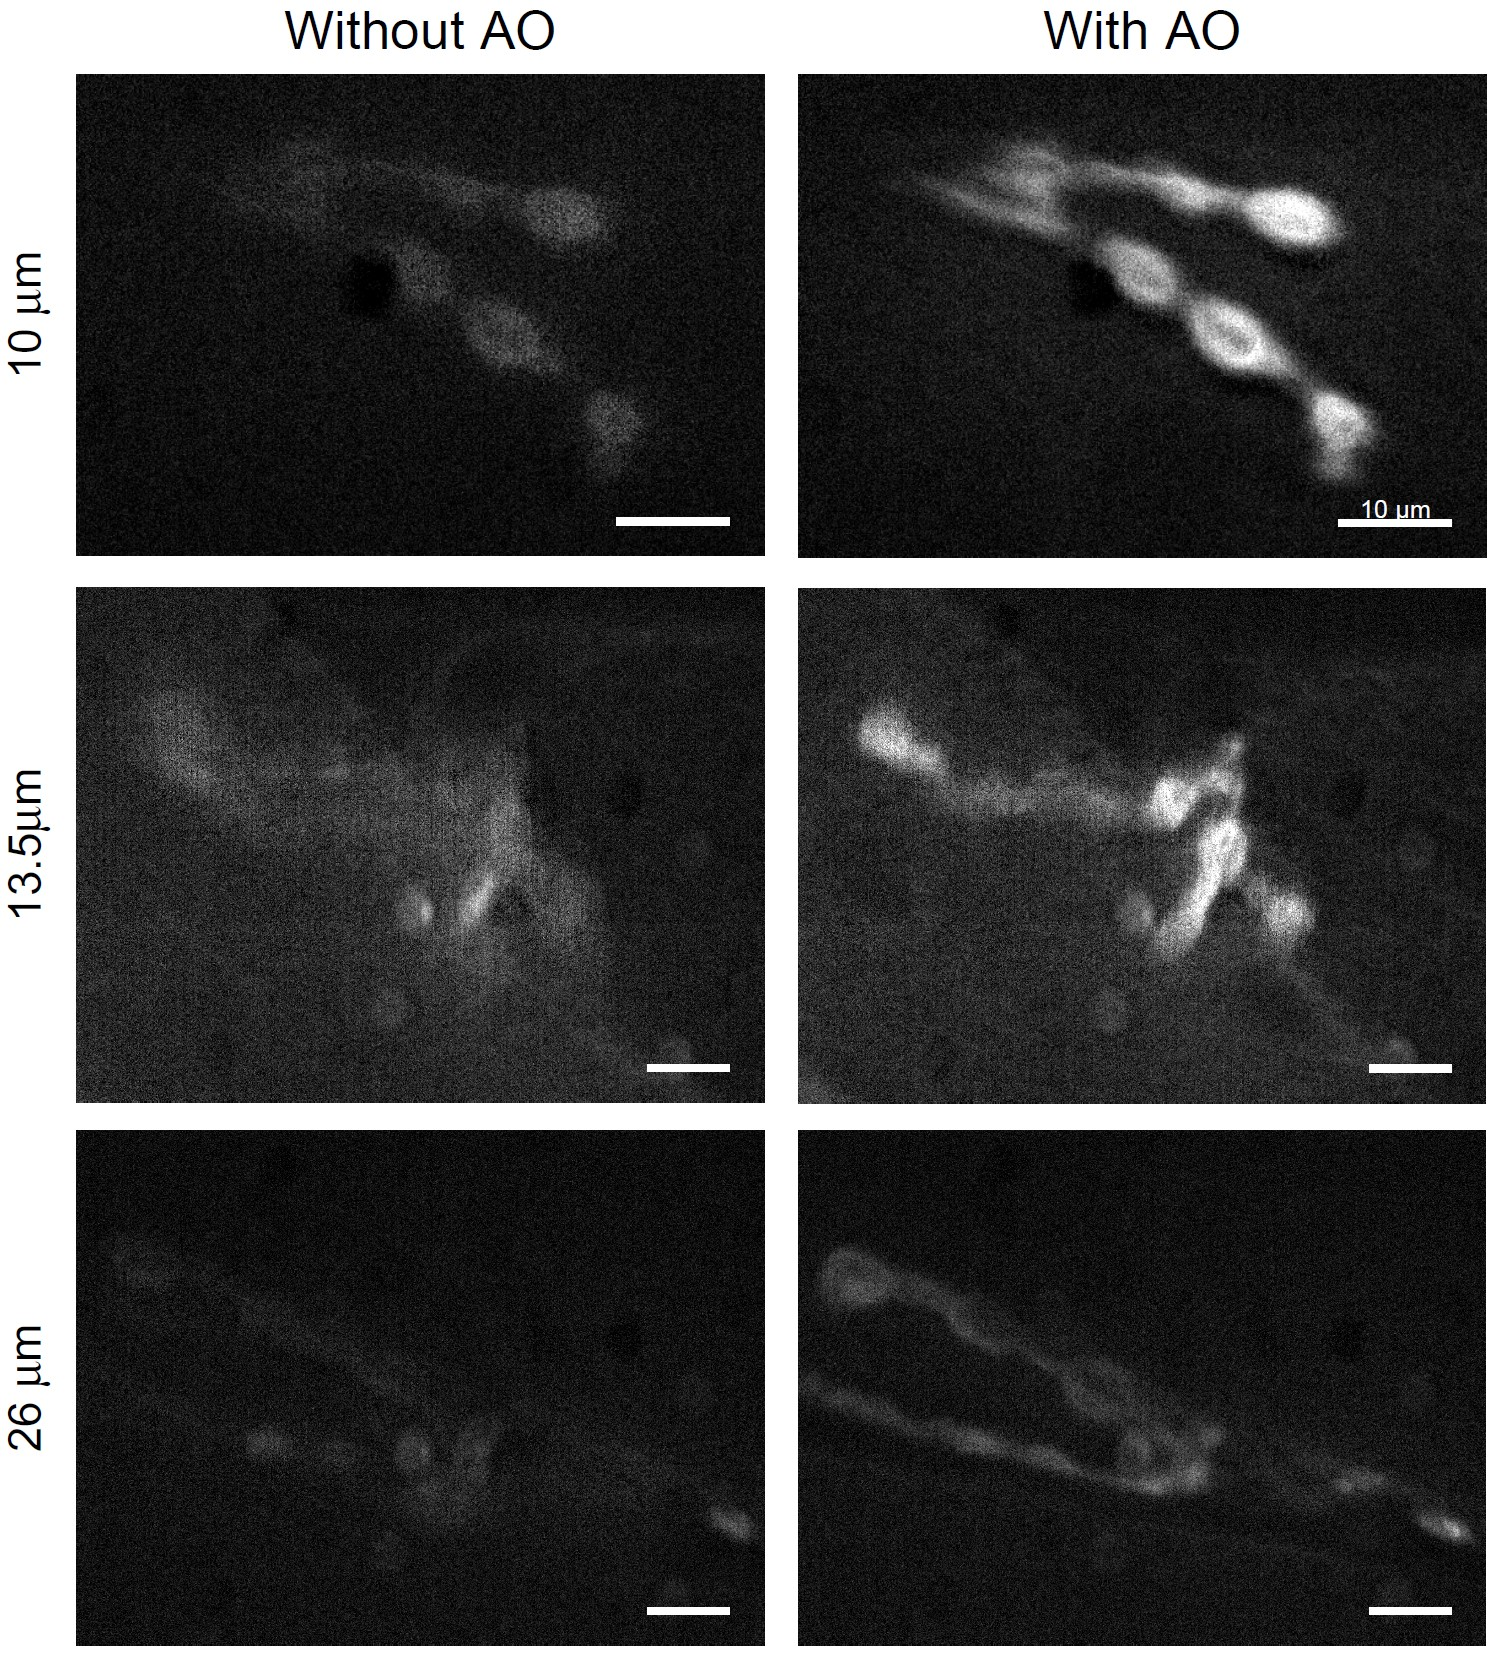
\includegraphics[width=\textwidth]{images/Aurox_depth_comparison_composite.jpg}
	\caption{Neuro-muscular junction images acquired at 10$\mu$m, 13.5$\mu$m 
		and 26$\mu$m with high optical sectioning. The images are of single 
		Z-positions. Aberration correction yields improvements in signal 
		and contrast at all depths. Scale bars are all 10$\mu$m. DLG signal 
		is shown. All images are displayed on the same intensity scale.}
	\label{fig:Aurox_depth_comparison_composite}
\end{figure}

Since the egg chambers samples were fixed and cleared, the sample induced 
aberrations were considerably less severe over a larger Z range. 
Figure~\ref{fig:Aurox_egg_chambers_composite} shows maximum intensity 
projections of 90$\mu$m Z-stacks obtained at high optical sectioning, both
without and with aberration correction. Ovarioles were separated out to 
better visualise individual egg-chambers Once again the overall contrast 
and intensity are improved with aberration correction. This is most 
noticable with the actin associated with ring-canals, pores which connect 
adjacent nurse cells and the oocyte to adjacent nurse cells the egg chamber.
In many of the cases highlighted in Figure~\ref{fig:Aurox_egg_chambers_composite}
with the arrows, the ring structure of these ring-canals is not visible
without aberration correction.

\begin{figure}[h]
	\centering
	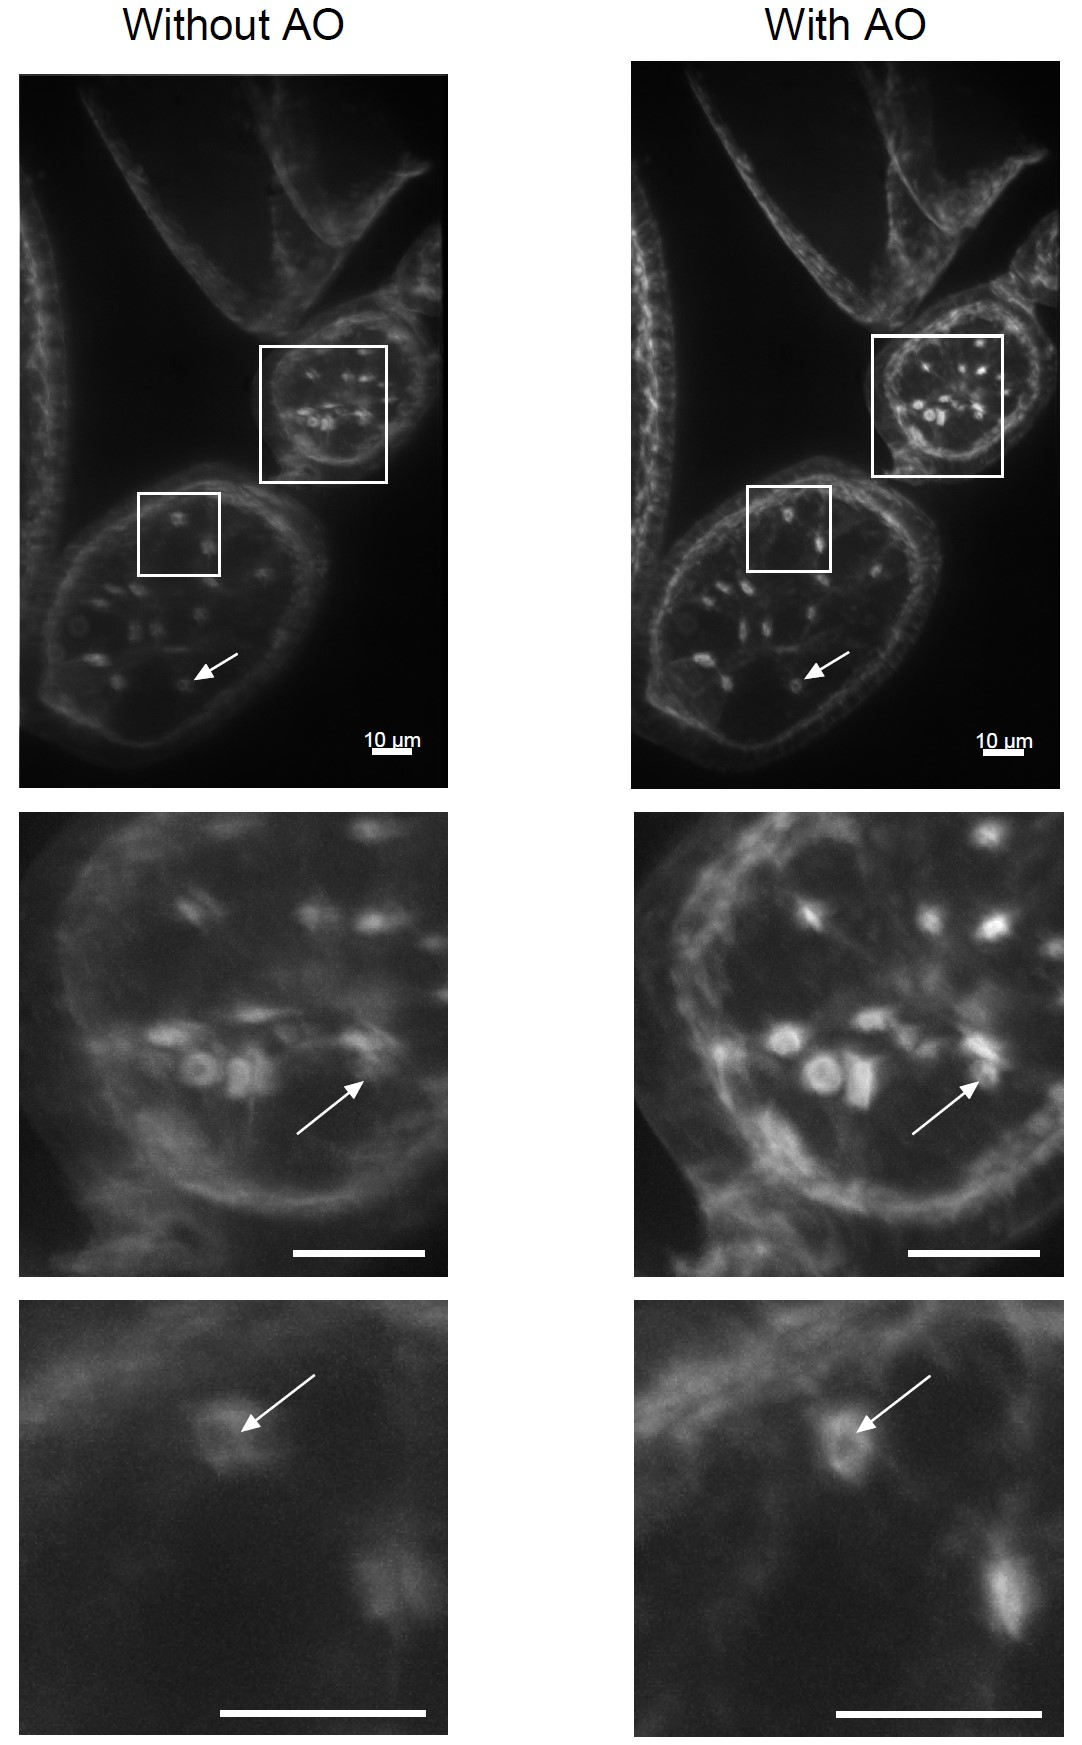
\includegraphics[width=0.8\textwidth]{images/Aurox_egg_chambers_composite.jpg}
	\caption{Maximum intensity projections of 90$\mu$m Z-stacks of egg 
		chamber samples acquired without (left) and with (right) adaptive 
		optics correction at high optical sectioning. The overall intensity 
		and contrast are improved after correction. The arrows highlight 
		particularly notable areas of improvement where fine details, such 
		as the outline of ring canals, become clearly visible. Scale bars 
		are all 10$\mu$m. Actin signal is shown. All images are displayed 
		on the same intensity scale.}
	\label{fig:Aurox_egg_chambers_composite}
\end{figure}

Finally, Figure~\ref{fig:Aurox_NMJ_composite_grey_and_color} shows maximum 
intensity projections of 20$\mu$m Z-stacks obtained at high optical 
sectioning, both without and with aberration correction. Despite the 
sensorless adaptive optics routine being performed only using the data 
from the Alexa 568 (HRP) channel, improvements in intensity and contrast
are observed in all imaging channels. Notably, the aberration correction 
allows for individual fibres in the segmental nerve to be resolved. Without
aberration correction the structure of individual round postsynaptic 
densities, boutons, are either unclear or not visible. Once the sample 
induced aberrations have been corrected, the structure of these boutons 
becomes clearer and the presence of several new, previously obscured, boutons 
can be observed.

\begin{figure}[h]
	\centering
	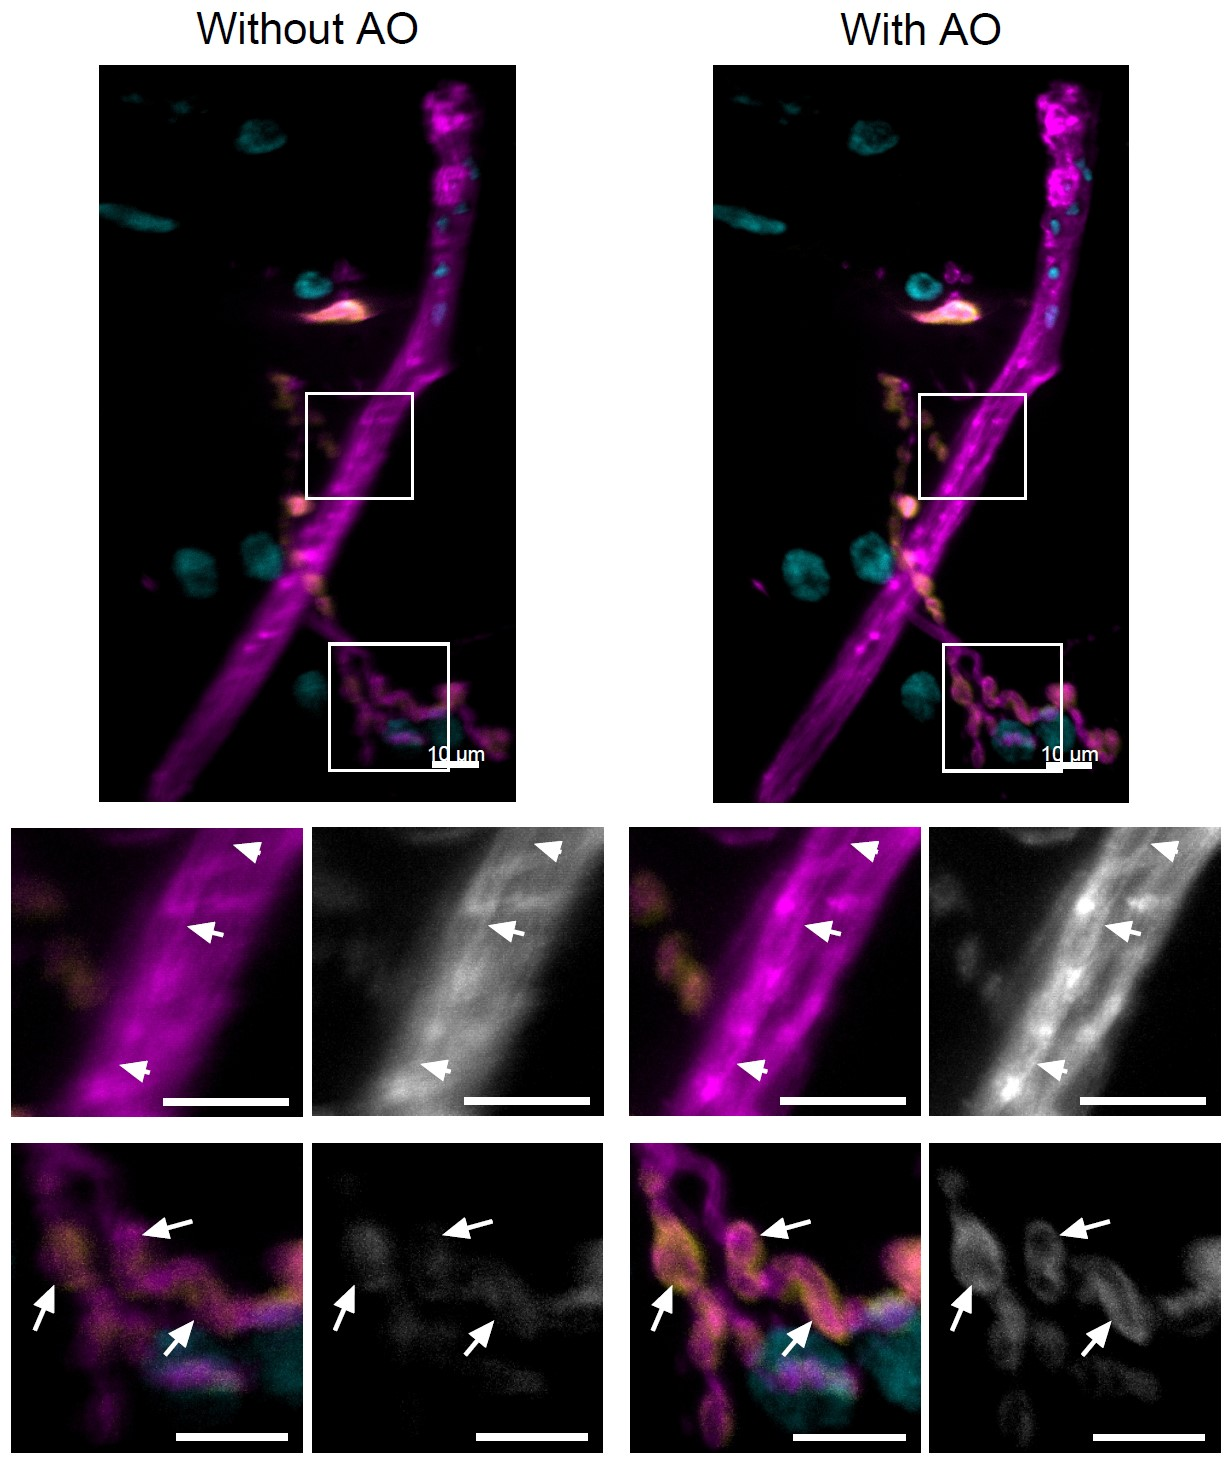
\includegraphics[width=\textwidth]{images/Aurox_NMJ_composite_grey_and_color.jpg}
	\caption{Maximum intensity projections of 20$\mu$m Z-stacks of 
		neuro-muscular junction samples acquired without (left) and with 
		(right) adaptive optics correction at high optical sectioning. 
		DLG shwon in yellow, HRP shown in magenta, nuclei shown in cyan. 
		Middle row greyscale images show only HRP. Bottom row greyscale 
		images show only DLG. The overall intensity and contrast are 
		improved after correction. The arrows highlight particularly 
		notable areas of improvement where fine details, such as 
		individual nerve fibers, become clearly visible. Scale bars are 
		all 10$\mu$m. All images are displayed on the same intensity 
		scale.}
	\label{fig:Aurox_NMJ_composite_grey_and_color}
\end{figure}
